\documentclass[12pt]{article}

\usepackage[utf8]{inputenc}
\usepackage{amsmath,amsthm,amsfonts,amssymb,amscd}
\usepackage{multirow,booktabs}
\usepackage[table]{xcolor}
\usepackage{fullpage}
\usepackage{lastpage}
\usepackage{enumitem}
\usepackage{fancyhdr}
\usepackage{mathrsfs}
\usepackage{wrapfig}
\usepackage{setspace}
\usepackage{calc}
\usepackage{multicol}
\usepackage{cancel}

\usepackage{graphicx}
%%\usepackage{caption}
%%\usepackage{subcaption}


\usepackage{listings}
\usepackage{matlab-prettifier}
\usepackage[framed,numbered,autolinebreaks,useliterate]{mcode}

\usepackage[margin=3cm]{geometry}
\newlength{\tabcont}
\setlength{\parindent}{0.0in}
\setlength{\parskip}{0.05in}
\usepackage{empheq}
\usepackage{framed}
\usepackage[most]{tcolorbox}
\usepackage{xcolor}
\colorlet{shadecolor}{orange!15}
\parindent 0in
\parskip 12pt
\geometry{margin=1in, headsep=0.25in}
\usepackage{float}
\usepackage{graphicx}
\usepackage{hyperref}


\newtheorem{thm}{Theorem}
\theoremstyle{theorem}
\newtheorem{reg}{Rule}
\newtheorem{exe}{Exercise}
\newtheorem{rem}{Remark}
\newtheorem{cor}{Corollary}
\newtheorem{exa}{Example}
\newtheorem{defi}{Definition}

\usepackage{natbib}
\bibliographystyle{abbrv}

\usepackage{times}
%\usepackage[compact]{titlesec}
\usepackage{titlesec}
\titlespacing*{\section}{0pt}{*-2}{*-1}
\titlespacing*{\subsection}{0pt}{*-2}{*-1}
\titlespacing*{\subsubsection}{0pt}{*-2}{*-1}

\def\a{\alpha}
\def\b{\beta}
\def\de{\delta}
\def\De{\Delta}
\def\ga{\gamma}
\def\Si{\Sigma}
\def\si{\sigma}
\def\ep{\varepsilon}
\def\ze{\zeta}
\def\om{\omega}
\def\leq{\leqslant}
\def\rar{\rightarrow}
\def\Rar{\Rightarrow}
\def\td{\Leftrightarrow}
\def\R{\hro{R}}
\def\C{\hro{C}}
\def\hro{\mathbb}
\def\bbI{\hro{I}}
\def\N{\hro{N}}
\def\Z{\hro{Z}}

\def\tE{\tilde{E}}
\def\hE{\hat{E}}
\def\tA{\tilde{A}}
\def\tT{\tilde{T}}
\def\hA{\hat{A}}
\def\hD{\hat{D}}
\def\bA{\breve{A}}
\def\tB{\tilde{B}}
\def\hB{\hat{B}}
\def\tC{\tilde{C}}
\def\tN{\tilde{N}}
\def\hN{\hat{N}}
\def\tk{\tilde{k}}
\def\tX{\tilde{X}}
\def\hX{\hat{X}}
\def\bX{\breve{X}}
\def\tM{\tilde{M}}
\def\tm{\tilde{m}}
\def\bM{\breve{M}}
\def\hM{\hat{M}}
\def\bm{\breve{m}}
\def\tH{\tilde{H}}
\def\tF{\tilde{F}}
\def\tG{\tilde{G}}
\def\hG{\hat{G}}
\def\tK{\tilde{K}}
\def\tx{\tilde{x}}
\def\tf{\tilde{f}}
\def\hf{\hat{f}}
\def\brf{\breve{f}}
\def\baf{\bar{f}}
\def\tg{\tilde{g}}
\def\hg{\hat{g}}
\def\lb{\lambda}
\def\cP{{\cal P}}
\def\cQ{{\cal Q}}
\def\fr{\frac}
\def\frQ{\mathfrak{Q}}

\def\cU{{\cal U}}
\def\cV{{\cal V}}
\def\cH{{\cal H}}
\def\tcU{{\tilde{\cal U}}}
\def\cZ{{\cal Z}}

\def\hxi{\widehat{\xi}}
\def\hp{\hat{q}}

\def\ddt{\fr{\mathrm{d}}{\mathrm{d}t}}
\def\dtau{\Delta_{\tau}}
\def\tnu{\tilde{\nu}}
\def\tU{\tilde{U}}

\def\tcQ{{\tilde{\cal Q}}}
\def\tcP{{\tilde{\cal P}}}
\def\hcP{\widehat{\cP}}
\def\hcQ{\widehat{\cQ}}
\def\cE{\mathcal{E}}
\def\cA{\mathcal{A}}
\def\cD{\mathcal{D}}
\def\hcE{\hat{\cE}}
\def\hcA{\hat{\cA}}
\def\hcD{\hat{\cD}}
\def\vphi{\varphi}

\newcommand{\n}[1]{\left\lVert#1\right\rVert}

\newcommand{\m}[1]{
	\begin{bmatrix}
		#1
	\end{bmatrix}
}

\renewcommand{\pm}[1]{
	\begin{matrix}
		#1
	\end{matrix}
}

\def\ES{
	\begin{bmatrix}
		J^E  & 0        & 0       & 0 \\
		0       & N^E_{2} & 0       & 0 \\
		0       & 0        & N^E_{3}& 0 \\
		0       & 0        & 0       & N^E_{4} 
	\end{bmatrix}
}

\def\AS{
	\begin{bmatrix}
		A_{1}  & 0       & 0          &  0        \\
		0           & J^A  & 0          & 0      \\
		0           &   0                & N^A_{3}      & 0      \\
		0           &   0                & 0                    & N^A_{4}      
	\end{bmatrix}
}
\def\BS{
	\begin{bmatrix}
		B_{1}  & 0       & 0        & 0 \\
		0          & B_{2}       & 0        & 0 \\
		0          & 0                  & J^B  & 0  \\
		0          & 0                 &   0                & N^B_{4}  \\ 
	\end{bmatrix}
}

\def\be{\begin{equation}}
\def\ee{\end{equation}}         

\newcommand{\ben}{\begin{eqnarray}}
\newcommand{\een}{\end{eqnarray}}

\newcommand{\bens}{\begin{eqnarray*}}
\newcommand{\eens}{\end{eqnarray*}}

\def\bc{\begin{cases}}
\def\ec{\end{cases}}

\newcommand{\bsq}{\begin{subequations}}
\newcommand{\esq}{\end{subequations}}

\newcommand{\eproof}{\space
	{\ \vbox{\hrule\hbox{\vrule height1.3ex\hskip0.8ex\vrule}\hrule}}\\[0.2cm]}

\begin{document}
% \setcounter{section}{8} This is assumed that count from Section 9

\thispagestyle{empty}

\begin{center}
	{\LARGE \bf Chapter 6. Numerical Integration and Differentiation } \\[.2cm]
	{\large Numerical Analysis 1. Winter Semester 2018-19}
\end{center}

\section{Trapezoidal, Simpson and Midpoint rules}

\subsection{Trapezoidal rule}

\subsection{Error estimation}

\subsection{Simpson rule}

\subsection{Midpoint rule rule}

\section{Error analysis}

\subsection{For Trapezoidal rule}

\subsection{For Simpson rule}

\subsection{For Midpoint rule}

\cleardoublepage 

\section{Newton-Cotes formulae}

Newton-Cotes quadrature formulas for approximating $\int_{a}^{b} f(x) dx$ are obtained by approximating the function of integration $f(x)$ by interpolating polynomials. 
The rules are \emph{closed} when they involve function values at the ends of the interval of integration. Otherwise, they are said to be \emph{open}.

\begin{figure}[h!]
	\centering
	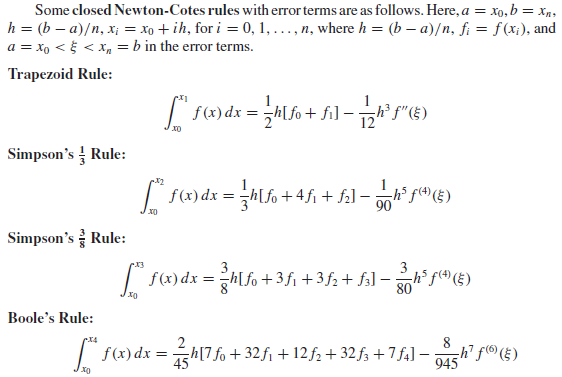
\includegraphics[scale=0.9]{Figures/44}
	\caption{\cite{BurF10},p.225}
	\label{fig:44}
\end{figure}

\begin{figure}[h!]
	\centering
	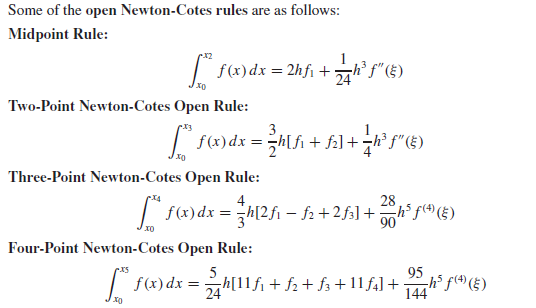
\includegraphics[scale=0.9]{Figures/45}
	\caption{\cite{BurF10},p.226}
	\label{fig:45}
\end{figure}

Over the years, many Newton-Cotes formulas have been derived and are compiled in
the handbook by Abramowitz and Stegun [1964], which is available online. Rather than
using high-order Newton-Cotes rules that are derived by using a single polynomial over
the entire interval, it is preferable to use a composite rule based on a low-order basic
Newton-Cotes rule. There is seldom any advantage to using an open rule instead of a closed
rule involving the same number of nodes. Nevertheless, open rules do have applications in
integrating a function with singularities at the endpoints and in the numerical solution of
ordinary differential equations as discussed in Chapter 10 and 11.\\
Before the widespread use of computers, the Newton-Cotes rules were the most commonly
used quadrature rules, since they involved fractions that were easy to use in hand
calculations. The Gaussian quadrature rules of the next section use fewer function evaluations
with higher-order error terms. The fact that they involve nodes involving irrational
numbers is no longer a drawback on modern computers.

\cleardoublepage 

\section{Romberg Quadrature Formulas}

\cleardoublepage

\section{Gaussian Quadrature Formulas}

\begin{figure}[h!]
	\centering
	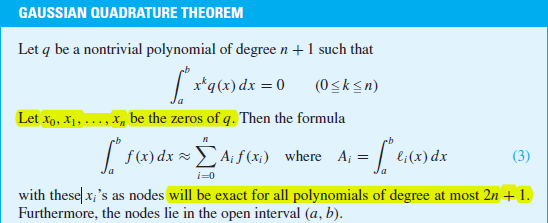
\includegraphics[scale=1.0]{Figures/46}
	\caption{\cite{CheK07},p.233}
	\label{fig:46}
\end{figure}

\begin{shaded}
With arbitrary nodes, Formula (3) will be exact for all polynomials of degree $\leq n$. With the Gaussian nodes, Formula (3) will be exact for all polynomials of
degree $\leq 2n + 1$.
\end{shaded}

\begin{figure}[h!]
	\centering
	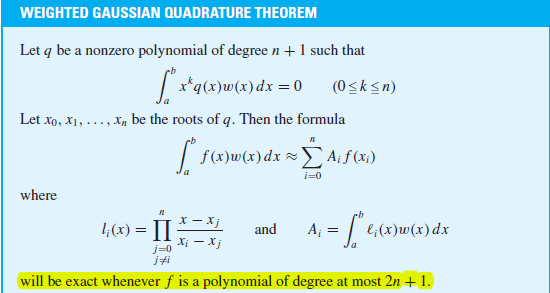
\includegraphics[scale=1.0]{Figures/47}
	\caption{\cite{CheK07},p.235}
	\label{fig:47}
\end{figure}

\cleardoublepage

\begin{figure}[h!]
	\centering
	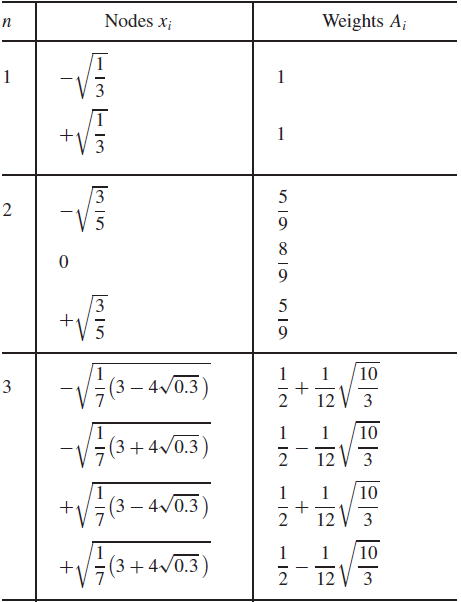
\includegraphics[scale=0.8]{Figures/48}
	\caption{Gaussian Quadrature Nodes and Weights, \cite{CheK07},p.235}
	\label{fig:48}
\end{figure}

\begin{figure}[h!]
	\centering
	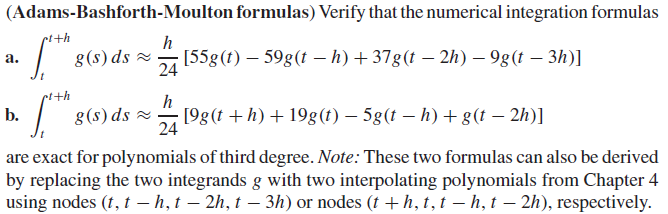
\includegraphics[scale=0.8]{Figures/50}
	\caption{\cite{CheK07},p.241}
	\label{fig:50}
\end{figure}

\begin{shaded}
 Gaussian numerical integration is not as simple to use as are the trapezoidal and Simpson rules, partly because the Gaussian nodes and weights do not have simple formulas and also because the error is harder to predict. Nonetheless, the increase in the speed of convergence is so rapid and dramatic in most instances that the method should 
 always be considered seriously when one is doing many integrations. Estimating the error is quite difficult, and most people satisfy themselves by looking at two or more 
 successive values. If n is doubled, then repeatedly comparing two successive values, $I_n$, and $I_{2n}$, is almost always adequate for estimating the error in $I_n$
%
\[ I-I_n \approx I_{2n} - I_n \ . \]%
This is somewhat inefficient, but the speed of convergence in 1,, is so rapid that this will still not diminish its advantage over most other methods. 
\end{shaded}

\subsection{Other Gaussian quadrature rules} 
Gauss-Kronrod, Curtis-...

\cleardoublepage

\section{Integrals with Singularities}
If either the interval of integration is unbounded or the function of integration is unbounded,
then special procedures must be used to obtain accurate approximations to the integrals.
One approach for handling a singularity in the function of integration is to change
variables to remove the singularity and then use a standard approximation technique.

\begin{figure}[h!]
	\centering
	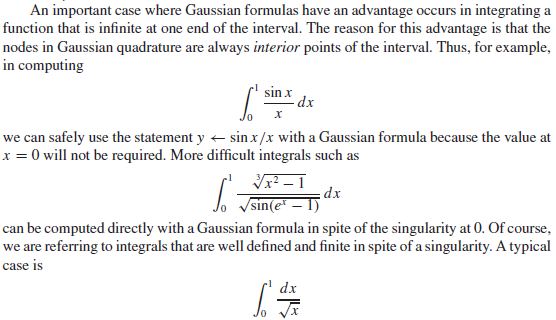
\includegraphics[scale=1.1]{Figures/49}
	\label{fig:49}
\end{figure}

\cleardoublepage
\section{Adaptive method}

\cleardoublepage
\section{What have not been covered?}

\begin{shaded}
In this script we have not considered the following topics.
\begin{enumerate}
 \item[i)] Rational Function Approximation, see \cite{BurF10}, Section 8.4. 
 \item[ii)] Trigonometric Polynomial Approximation, see \cite{BurF10}, Section 8.5. 
\end{enumerate}
\end{shaded}

\section{Survey of Methods and Software}
In this chapter we considered approximating data and functions with elementary functions.
The elementary functions used were polynomials, rational functions, and trigonometric
polynomials. We considered two types of approximations, discrete and continuous. Discrete
approximations arise when approximating a finite set of data with an elementary
function. Continuous approximations are used when the function to be approximated is
known.

Discrete least squares techniques are recommended when the function is specified by
giving a set of data that may not exactly represent the function. Least squares fit of data
can take the form of a linear or other polynomial approximation or even an exponential
form. These approximations are computed by solving sets of normal equations, as given in
Section 8.1.

If the data are periodic, a trigonometric least squares fit may be appropriate. Because
of the orthonormality of the trigonometric basis functions, the least squares trigonometric
approximation does not require the solution of a linear system. For large amounts of
periodic data, interpolation by trigonometric polynomials is also recommended. An efficient
method of computing the trigonometric interpolating polynomial is given by the fast
Fourier transform.

When the function to be approximated can be evaluated at any required argument,
the approximations seek to minimize an integral instead of a sum. The continuous least
squares polynomial approximations were considered in Section 8.2. Efficient computation
of least squares polynomials lead to orthonormal sets of polynomials, such as the Legendre
and Chebyshev polynomials. Approximation by rational functions was studied in Section
8.4, where Pad´e approximation as a generalization of the Maclaurin polynomial and its extension
to Chebyshev rational approximation were presented. Both methods allow a more
uniform method of approximation than polynomials. Continuous least squares approximation
by trigonometric functions was discussed in Section 8.5, especially as it relates to
Fourier series.

\newpage

\nocite{*}

\bibliography{GTS_reference} 

\end{document}